\documentclass[10pt, a4paper]{scrartcl}

\usepackage{vorschule}
\usepackage[
	typ=ab,
	fach=Mathematik,
	lerngruppe={Q2-GK},
	nummer=III.9,
	module={Symbole,Lizenzen},
	seitenzahlen=keine,
	farbig,
	lizenz=cc-by-nc-sa-4,
]{schule}

\usepackage[
	kuerzel=Ngb,
	reihe={Analytische Geometrie},
	version={2019-12-12},
]{ngbschule}

\author{J. Neugebauer}
\title{Winkel zwischen Vektoren}
\date{\Heute}

\setzeAufgabentemplate{ngbnormal}


\begin{document}
\ReiheTitel

\begin{infobox}
\begin{wrapfig}
	\begin{wrapfigure}[3]{r}{0pt}
		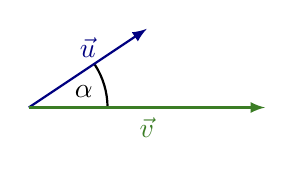
\begin{tikzpicture}[thick]
		\draw[draw=black] (0:1) arc (0:33:1);
		\draw[-latex,color=NavyBlue] (0,0) --node[above] {$\vec{u}$} (1.5,1);
		\draw[-latex,color=OliveGreen] (0,0) --node[below] {$\vec{v}$} (3,0);
		\node at (.7,.2) {$\alpha$};
		\end{tikzpicture}
	\end{wrapfigure}
	Für zwei Vektoren $\vec{u}\neq\vec{o}$ und 
	$\vec{v}\neq\vec{o}$ mit dem eingeschlossenen Winkel $\alpha$ gilt:
	\[ \vec{u}\ast\vec{v} = \abs{\vec{u}}\cdot\abs{\vec{v}}\cdot\cos{\alpha} \]
\end{wrapfig}
\end{infobox}

\begin{aufgabe}
	\operator{Berechnen} sie zunächst den Winkel zwischen den Vektoren $\vec{u}$ und $\vec{v}$\footnote{Die Umkehrfunktion des Kosinus ist $\operatorname{cos^{-1}}$ und ist auf dem GTR unter \menu{trig} zu finden. Es gilt dann \[ \cos{\alpha} = x \Leftrightarrow \alpha = \operatorname{cos^{-1}(x)}\]}. 
	
	\operator{Konstruieren} sie \emph{danach} die beiden Vektoren in GeoGebra und \operator{überprüfen} sie ihr Ergebnis.
	
	\begin{tasks}(2)
		\task \[ \vec{u} = \vector(2|-1|2) \qquad \vec{v} = \vector(4|0|-3) \]
		\task \[ \vec{u} = \vector(-3|-2|5) \qquad \vec{v} = \vector(7|1|-4) \]
	\end{tasks}
\end{aufgabe}

\begin{center}
\begin{minipage}{.9\textwidth}\begin{rahmen}\small
\subsubsection*{Konstruktionen in GeoGebra}
Erstellen sie in GeoGebra ein neues Dokument und aktivieren sie die \enquote{3D-Grafik} Ansicht.

GeoGebra bietet Werkzeuge zum Erstellen geometrischer Konstruktionen an. Schneller geht es aber oft,
die Konstruktion \enquote{von Hand} einzugeben. Dazu geben sie in der linken Seitenleiste von GeoGebra die folgenden Befehle ein:
\begin{description}
	\item[Punkte] Den Punkt \pkt[A](4|-5|3,6) erzeugen sie durch dei Eingabe \code{A = (4,-5,3.6)}.
	\item[Vektoren] Einene Vektor können sie auf zwei Arten erzeugen. Als \emph{Orstvektor} für einen Punkt (z.B. \code{v = Vektor(A)} oder \code{v = Vektor((1,2,3))}), oder als \emph{Differenzvektor} zwischen zwei Punkten (z.B. \code{u = Vektor(A, (4,5,7.2))}).
	\item[Winkel] Winkel können zwischen ganz verschiedenen Objekten erzeugt werden. Wichtig für uns 
	sind Winkel zwischen drei Punkten (z.B. \code{Winkel(A, B, (1,2,3))}) und zwischen zwei Vektoren (z.B. \code{Winkel(u, Vektor((4.5,6,8.2))}).
\end{description}
\end{rahmen}\end{minipage}
\end{center}

\begin{aufgabe}
	\operator{Ergänzen} sie die Formel zur Berechnung des Winkels zwischen zwei Vektoren.
	\medskip
	\begin{infobox}
		Für den Winkel $\alpha$ zwischen zwei Vektoren $\vec{u}\neq\vec{o}$ und 
			$\vec{v}\neq\vec{o}$ gilt:
			\[ \alpha = \hspace{4cm} \]
	\end{infobox}
\end{aufgabe}

\vspace{1cm}
\begin{aufgabe}[subtitle={Buch S.196, Afg.3}]
	\operator{Konstruieren} sie ein Modell der Situation in GeoGebra und \operator{ermitteln} sie den Winkel am Eckpunkt $C$. 
	
	
	\operator{Bestätigen} sie dann das Ergebnis \operator{rechnerisch}. 
\end{aufgabe}

\end{document}
